% Setup - do not change
\documentclass[11pt]{article}
\usepackage[top=0.9in, left=0.9in, bottom=0.9in, right=0.9in]{geometry} 
\usepackage{parskip}

\usepackage[english]{babel}
\usepackage[utf8]{inputenc}
\usepackage{amsmath,amsthm,amssymb,graphicx,pdfpages,lipsum,hyperref}
\usepackage{wrapfig}
\usepackage{subcaption}
\usepackage[none]{hyphenat}
\usepackage{csquotes}
\graphicspath{{plots/}}

\setlength\parindent{0pt}
%%%%%%%%%%%%%%%%%%%%%%%%%%%%%%%%%%%%%%%%%%%%%%%%%%%%%%%%%%%%%%%%%%%

%% Bibliography are specified in this file. You can also choose inline bib style if you want to. But make sure your citation style is consistent (and proper)
% For more details on citation: https://library.unimelb.edu.au/recite
\usepackage[sorting = none]{biblatex}
\addbibresource{references.bib}

%%%%%%%%%%%%%%%%%%%%%%%%%%%%%%%%%%%%%%%%%%%%%%%%%%%%%%%%%%%%%%%%%%% the '%' symbol denotes comments

% Begin document creation
% DELETE THE \lipsum PLACEHOLDERS WHEN YOU BEGIN
\title{\textbf{Predicting Yellow Taxi Demand with Public Transportation: Urban Mobility Insights}}
\author{
Ider Byambadorj \\
Student ID: 1198613 \\
%% Replace the link with your github repo
% 1. Remember to escape underscore (\_) in the link.
% 2. Remember to include the commit you want to submit in the link
\href{https://github.com/MAST30034-Applied-Data-Science/mast30034-project-1-iderbyambadorj/commit/80bbdb4091bab2fbb798cfe1722a49a88246dfd2}{Github repo with commit}
}

\begin{document}
\maketitle

\section{Introduction}

The relationship between public transport and taxi services has garnered the attention of many researchers, yet not a lot of research has been conducted on the topic. With the increased number of transport options, understanding the factors that shape the taxi demand is as important as ever. While previous studies have investigated the relationship between Uber and public transport services in New York City \cite{uber_public_transport}, the relationship between the yellow taxi and public transport remains an under-explored domain. 

In this project, we will use state-of-the-art machine learning and statistical modelling methodologies, including Random Forest Regressor and Linear Regression, to analyze the impact of public transport on taxi demands across different neighbourhoods in New York City. By doing so, we aim to provide insights for urban planners and taxi companies, helping them optimize traffic management in New York City.

\subsection{Dataset}
\subsubsection{TLC Taxi Trip Record Data}

The main dataset was collected from the New York City Taxi \& Limousine Commission Taxi Trip Record Data \cite{taxi_data}. Yellow taxi data from 2022 Jan 1st to 2023 May 31st were collected. The dataset included \textbf{55'842'484} instances with 19 features. The models will be trained on 2022 data, and tested on 2023 data.

Additionally, taxi zone data published from TLC has been used to aid our research. The taxi zone data included name, area and location information for all 263 taxi zones.

\subsubsection{Public Transport Data}

As our external spatial data, public transport data from Metropolitan Transportation Authority (MTA) was used \cite{mta_data}. Using Python script, we were able to extract all public transport stops information for each taxi zones represented. In total, 17638 stops were extracted.

\section{Preprocessing}

The preprocessing section consists of four phases: \textit{Data Wrangling, Feature Selection, Feature Engineering} and \textit{Aggregation}.

\subsection{Data Wrangling}

\begin{itemize}
  \item All instances with negative values of features were removed from the dataset. Although we are dropping some features later on, it is deemed useful to remove negative values for all features. The negative value in a feature may refer to an incorrect entry of trip data, thus making the data untrustworthy. A total of 2'406'872 ($\approx4.31\%$) instances were removed in this step.
  \item According to New York City Taxi \& Limousine Commission, the maximum number of passengers allowed in a taxi is 4. Therefore, all instances outside the range of 1 and 4 were removed from the dataset. 2'533'505 instances ($\approx4.74\%$) were outside the range and thus were removed.
  \item Trips with unusually small or large distances were removed. In this case, we have decided to remove trips that travelled less than 0.1 miles as it is within walking distance. On the other hand, we had an upper bound of 50 miles trip distance. Considering the distance between Staten Island and the Bronx, the two farthest boroughs in New York City, is about 37 miles, the maximum distance of 50 miles were placed. A total of 721'691 instances ($\approx1.41\%$) were removed.
  \item At last, all instances that had incorrect location\_id, and out-of-range dates were removed. 1'286'295 ($\approx2.56\%$)instances were removed in this step.
\end{itemize}

After filtering the dataset, we have a total of \textbf{48'894'121} instances. 

\subsection{Feature Selection, Feature Engineering}

Considering its relevance to our research question and timeline, any features specific to each trip, including fare features, were removed. The pick-up and drop-off times were then converted into the nearest hour. We then extracted days of the week, season and year information. In addition, we have separated the airport zone from the other zones in the borough. Since airport zones are abnormalities, it might be useful to put them in a separate class ``Airport'' as they are likely to share the same characteristics. This was done by changing the borough value for the airport zones to ``Airport''.

\subsection{Aggregation}

No missing values were seen at this stage. After performing the Feature Engineering, we grouped the dataset by location, hour, day, season, year as well as borough and summed over the pickup and drop-off counts. After grouping the data, we have \textbf{129'673} instances for pickup data and \textbf{231'563} instances for drop-off data with 6 features each. 

\subsection*{Public Transport Dataset}

After removing duplicates, the public transport dataset was joined to the taxi zone dataset by its location. After aggregating the data, we were able to find out the number of public transport stops for each taxi zones. This dataset was then joined to the taxi dataset on the taxi zone location id. From the public transport dataset, the following features were attained: 
\begin{itemize}
    \item \textbf{num\_stops} (Number of stops in a particular zone)
    \item \textbf{Shape\_Area} (Total area for the zone). This area was not converted to miles squared or kilometres squared because the area was calculated using the latitude and longitude of the zone. Based on the latitude, one degree of longitude would represent different lengths on Earth. Therefore, the Shape\_Area variable wasn't transformed to keep the area consistent.
\end{itemize}

After joining the public transport dataset and TLC taxi dataset, we have 129'673 instances and 9 features (including target feature) for pickup data, 231'563 instances and 9 features for drop-off data. 

\section{Preliminary Analysis}

Before training the model, it is crucial to learn the distributions of the data and do Exploratory Data Analysis. The following section will map different relationships that exist between different features. Since our training data covers the year 2022, the following set of analyses was done on the 2022 data.

\subsection{Distribution of the Taxi Data}

Based on our analysis, we have discovered that the distribution of pickup and drop-off counts is highly skewed. The number of pickups and drop-offs for different boroughs is very different, making the data imbalanced. 

\begin{figure}[h]
    \begin{subfigure}{0.5\textwidth}
        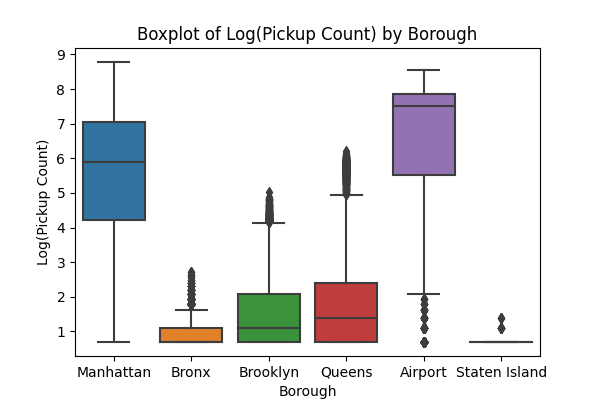
\includegraphics[width=0.9\linewidth]{boxplot_log_pickup.png} 
        \caption{Pickup}
        \label{fig:boxplot1}
    \end{subfigure}
    \begin{subfigure}{0.5\textwidth}
        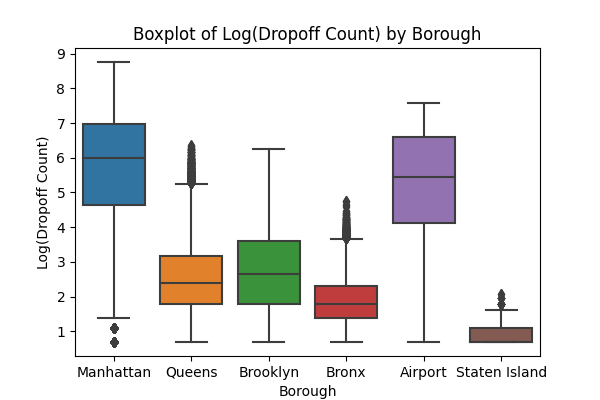
\includegraphics[width=0.9\linewidth]{boxplot_log_dropoff.png}
        \caption{Drop-off}
        \label{fig:boxplot2}
    \end{subfigure}
\caption{Distribution of Taxi Demand by Borough}
\label{fig:boxplot}
\end{figure}

From Figure \ref{fig:boxplot1}, the three most popular boroughs for taxi pickups are Airport, Manhattan and Queens. Meanwhile, Figure \ref{fig:boxplot2} shows that Manhattan, Airport and Brooklyn are the three most popular regions for taxi drop-offs. Based on the difference in spatial characteristics and the number of taxi pickups and drop-offs, we conclude that the relationship between public transport and taxi demand should be examined separately by borough. 

\subsection{Spatial Distribution}

\begin{figure}[h]
    \begin{subfigure}{0.5\textwidth}
        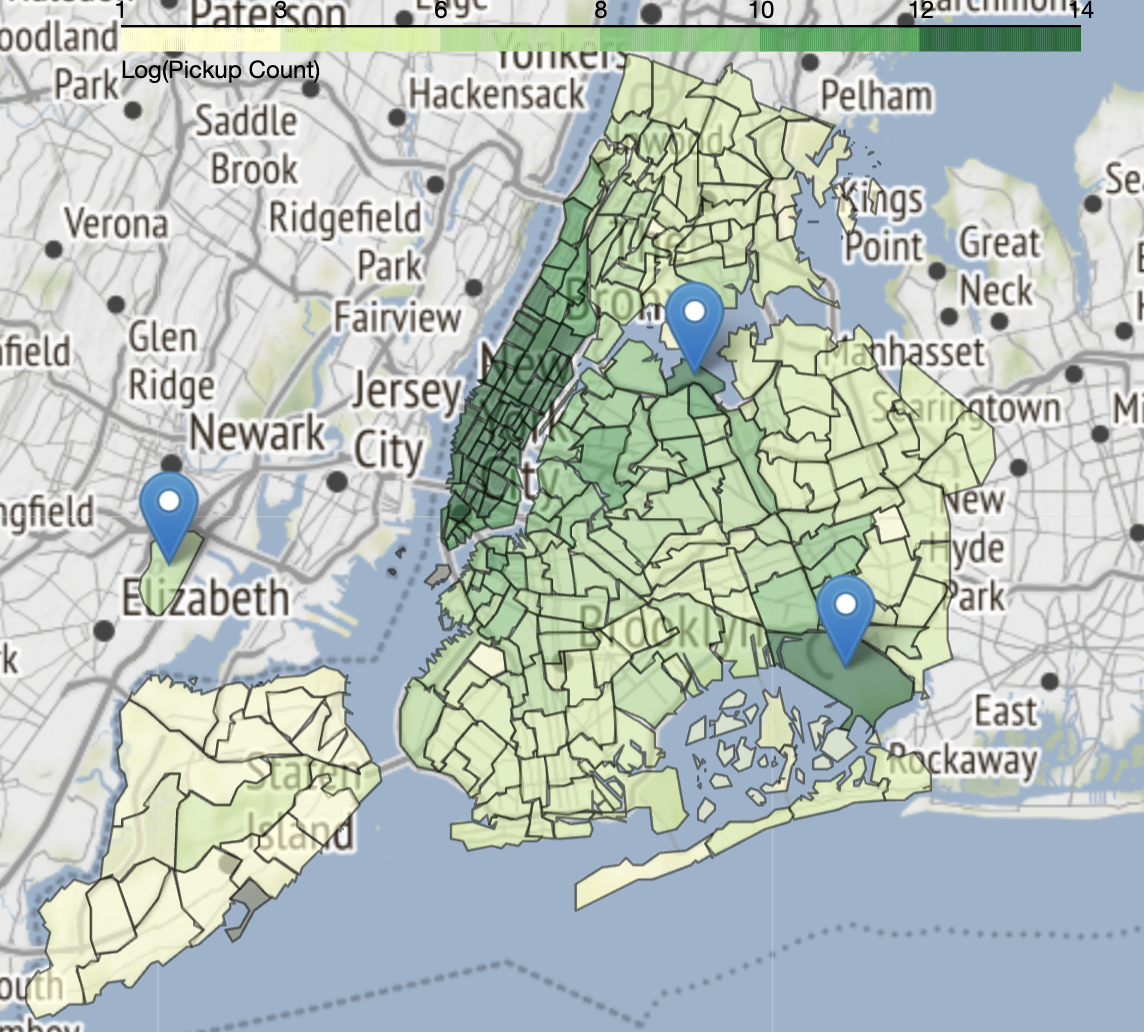
\includegraphics[width=0.9\linewidth, height=6cm]{pickup_choropleth.png} 
        \caption{Pickup}
        \label{fig:pickup_choropleth}
    \end{subfigure}
    \begin{subfigure}{0.5\textwidth}
        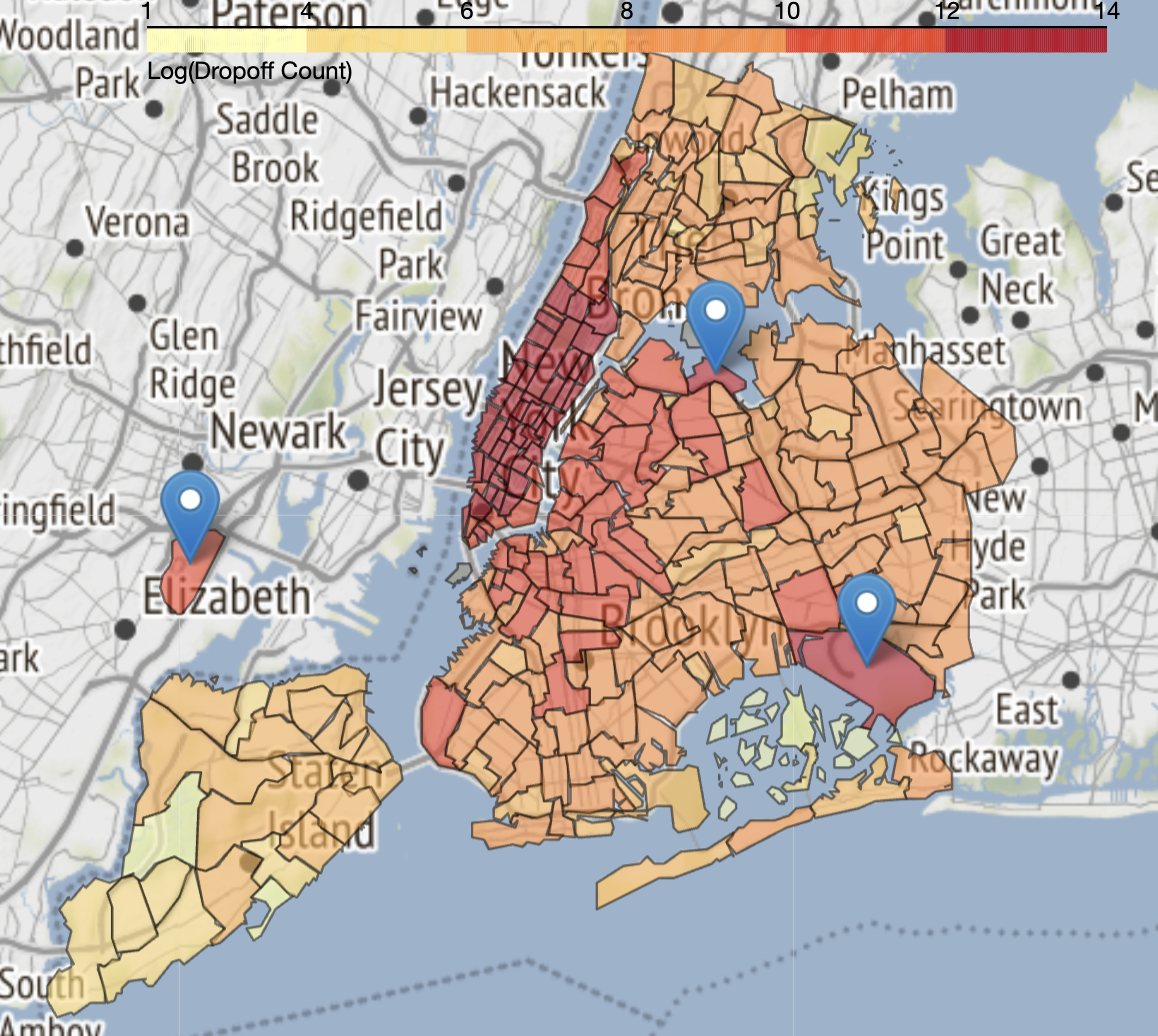
\includegraphics[width=0.9\linewidth, height=6cm]{dropoff_choropleth.png}
        \caption{Drop-off}
        \label{fig:dropoff_choropleth}
    \end{subfigure}
\caption{Distribution of Pickup and Drop-off counts}
\label{fig:taxi_choropleth}
\end{figure}

Since the dataset is highly skewed, we took the logarithm of the pickup and drop-off count to visualize the dataset. Figure \ref{fig:taxi_choropleth} shows us the distribution of total taxi pickup and drop-off counts. While the pickup data is more skewed towards the JFK airport and Manhattan borough, the drop-off distribution looks more evenly distributed with a high number of drop-offs at Brooklyn after JFK airport and Manhattan.

\subsection{Temporal Patterns}

While location may be an important factor, we have found that temporal features play an equally important part in the difference in taxi demands. According to Figure \ref{fig:lineplot_demand}, 3 pm to 7 pm are the most popular hours. We can see that the taxi demand is dependent on the day of the week. To elaborate, Wednesdays to Fridays are the most popular days, while Mondays and Sundays are the least popular days in terms of taxi demands. Figure \ref{fig:lineplot_demand} illustrates that demand changes across different seasons. Taxi demands reach their highest during Spring, and the lowest during Winter. To sum up, taxi demands clearly depend on temporal data, including hours, days and seasons.

\begin{figure}
    \centering
    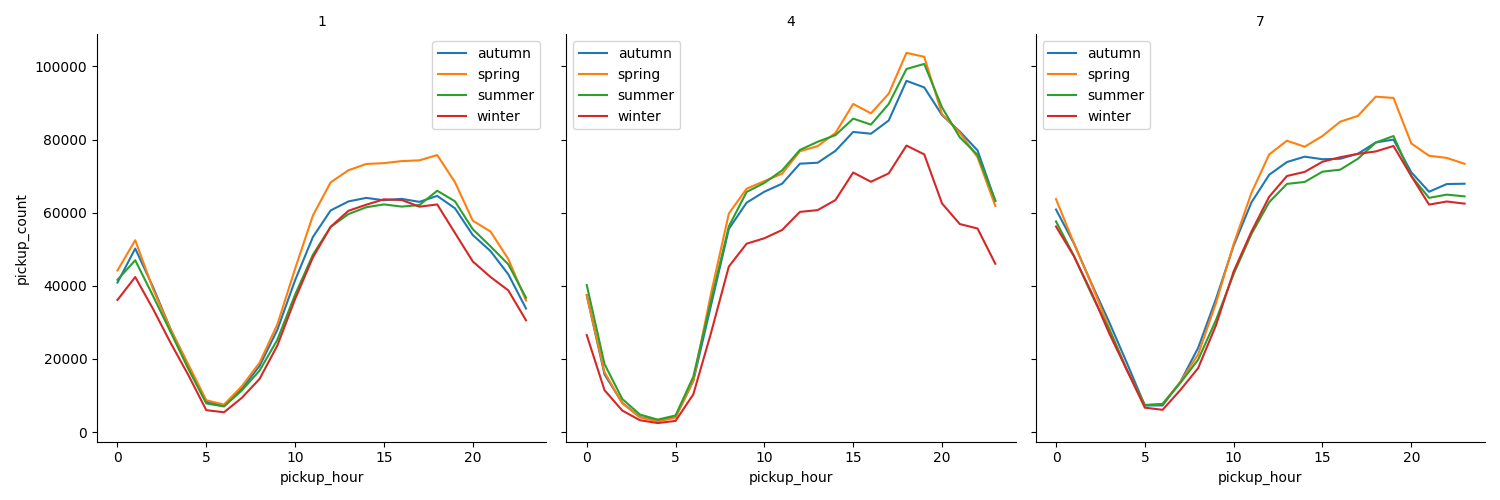
\includegraphics[width=\textwidth]{line_plot_pickup_count.png}
    \caption{Plot of total Taxi demand on different days during the week}
    \label{fig:lineplot_demand}
\end{figure}

\subsection{Public Transport}

Before training any models, it is important to find the distribution of the data and map any relationships between taxi data and public transport data.

\subsubsection{Correlation}

The correlation matrix can help us figure out the general pattern behind the relationship between the target variable and public transport features. 

\begin{figure}[h]
    \begin{subfigure}{0.48\textwidth}
        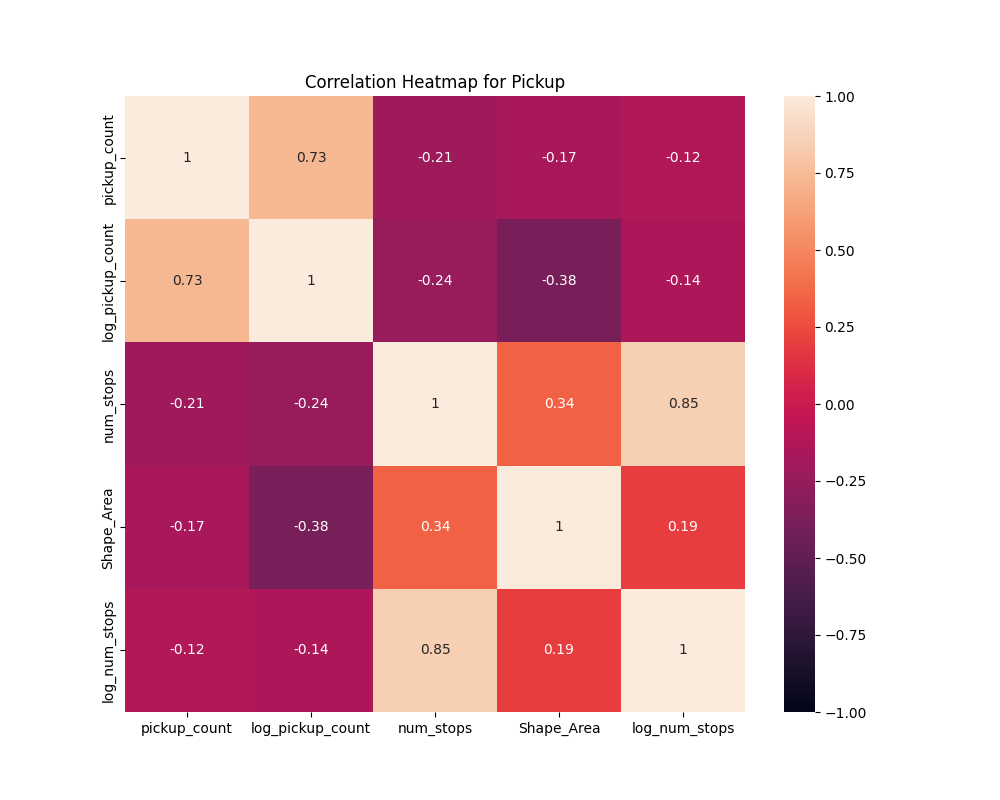
\includegraphics[width=\linewidth]{correlation_matrix_pickup.png} 
        \caption{Pickup}
        \label{fig:corr_pickup}
    \end{subfigure}
    \begin{subfigure}{0.48\textwidth}
        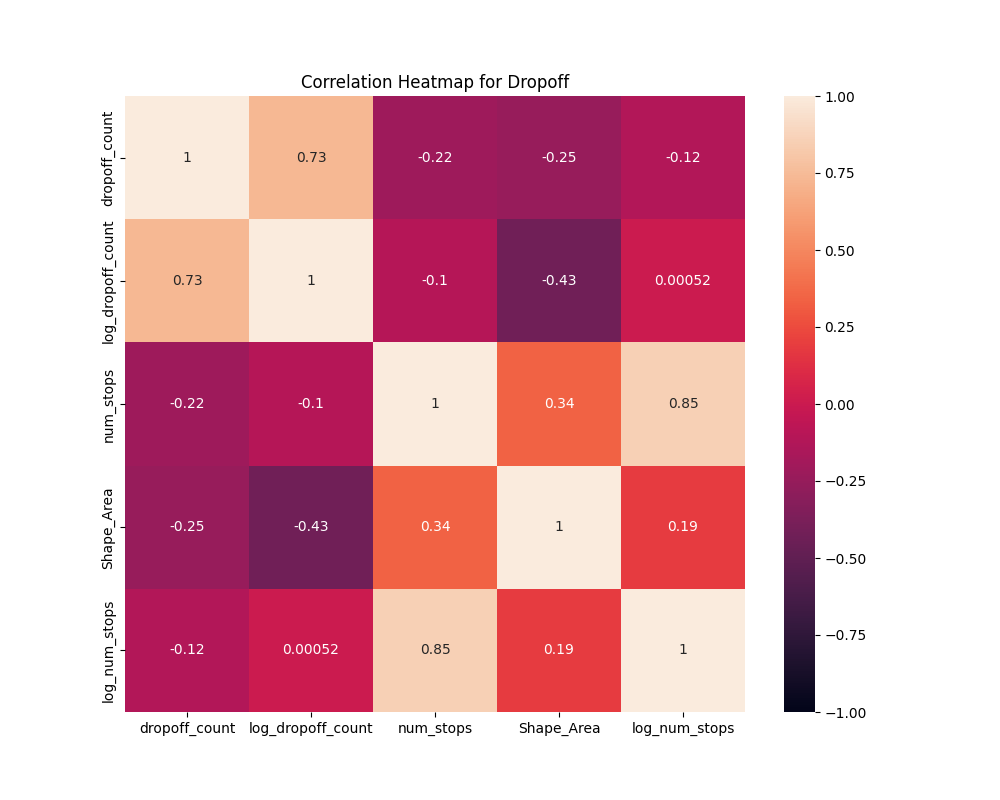
\includegraphics[width=\linewidth]{correlation_matrix_dropoff.png}
        \caption{Drop-off}
        \label{fig:corr_dropoff}
    \end{subfigure}
\caption{Correlation Matrix between Pickup, Drop-off and Public Transport Data}
\label{fig:corr_matrix}
\end{figure}

Figure \ref{fig:corr_pickup} shows us that pickup count and log(pickup count) are negatively related to the number of public transport stops with Pearson's correlation coefficient of -0.21 and -0.24 respectively. This negative relationship suggests that Public Transport and Taxi services are likely to compete in some areas. A similar characteristic can be shown in Figure \ref{fig:corr_dropoff}, where the drop-off count is negatively correlated with the number of public transport stops in the area with a coefficient of -0.22. 

\subsubsection{Distribution}

\begin{figure}[h]
  \centering
  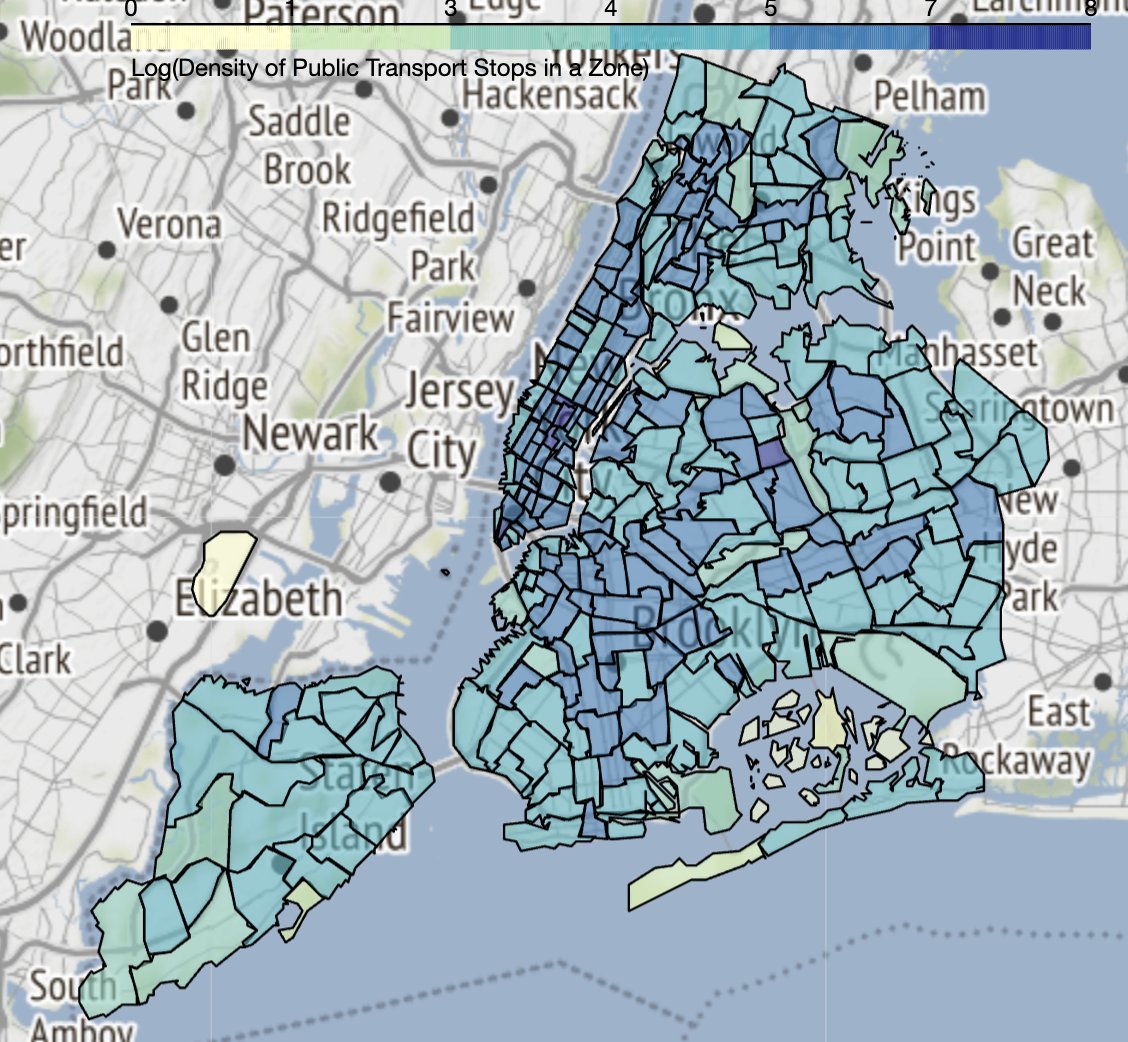
\includegraphics[width=0.5\linewidth]{public_transport.png} 
  \caption{Distribution of Public Transport Stops}
  \label{fig:public_transport}
\end{figure}

Similar to the distribution of taxi data, public transport data is skewed as well. As most public transport stops have to be within certain distances of each other, it makes the number of stops within a zone highly correlated to the total area of the zone. Since larger zones tend to have more stops, we calculated the density of stops by dividing the number of stops by the total area of the zone.

From Figure \ref{fig:public_transport}, we can see that Manhattan and Brooklyn have the highest densities for public transport stops. According to \ref{fig:public_transport}, the density of public transport density decreases as it gets farther from the city centre (Manhattan). Similar behaviour can be seen from the taxi demand distribution. 

\section{Modelling}

This section covers the two regression models used in this project: Linear Regression and Random Forest Regression.

Mean Absolute Error (MAE) was used as our performance evaluation method for the two models. MAE calculates the error by averaging the absolute error for the prediction. Unlike Root Mean Squared Errors (RMSE), MAE won't be biased towards data points with large values. Since our dataset is skewed and has many outliers, MAE is more suitable than RMSE in this case.

\subsection{Linear Regression}

Linear regression is a statistical approach that aims to identify linear associations between input features and a target variable, making it suitable for capturing simple correlations. 

\begin{table}[]
\centering
\begin{tabular}{|l|c|c|}
              & Number of instances & R-squared \\
Airport       & 1501                & 0.927     \\
Bronx         & 6565                & 0.431     \\
Brooklyn      & 18093               & 0.665     \\
Manhattan     & 40968               & 0.899     \\
Staten Island & 198                 & 0.244     \\
Queens        & 19133               & 0.795    

\end{tabular}
\caption{Number of instances and R-squared for Linear Regression model on Pickup}
\label{tab:lr_result}
\end{table}

To account for the difference in relationships and data distribution, different linear models were trained for each borough in the data. According to the diagnostic plots, there were signs of heteroskedasticity in the model. This is an indication of non-linear relationships between the target variable and dependent variables. We then transformed the dependent variable by taking a natural logarithm. This allows us to retain the relationships while avoiding multiplicative errors \cite{mast30025}

As linear regression is prone to outliers, we have removed outliers by calculating its cook's distance. Cook's distance is an estimation of an influence of a data point in the model. Data points with high Cook's distance are likely to affect the fit of the model greater than other points. A total of 3112 data points were removed from the pickup dataset.

After careful analysis and feature selection, the following model was chosen as the final model: \[Y=X\beta + \epsilon\] where $Y$ is the log-transformed count, $X$ is a vector containing the features: location\_id, hour, day, season, number of stops and zone area, $\beta$ is a vector containing coefficients of the linear model and $\epsilon$ is the error/residuals. 

\subsection{Random Forest Regression}

Random Forest Regression uses an ensemble learning method for regression \cite{comp30027}. It fits a number of decision trees and aggregates their result to predict the target variable. Compared to Linear Regression, RFRegression is able to capture complex non-linear relationships in the data.

We have trained the RFR in 6 different boroughs: Airport, Bronx, Brooklyn, Manhattan, Staten Island and Queens. Before training the model, additional preprocessing had to be done:
\begin{itemize}
    \item One-Hot-Encode all categorical features, including location\_id, hour, day and season.
    \item Standardize all data using StandardScaler from scikit-learn. This ensures all variables contribute equally to the target variable.
    \item Split the data into training and test data. We trained the RFRegressor on 2022 data and tested the model on 2023 data.
\end{itemize}

In order to improve the performance, we tuned the hyperparameters using GridSearchCV from scikit-learn. In GridSearch, Root Mean Squared Error (RMSE) was used as the evaluation method. 

\begin{figure}[h]
   \begin{minipage}{0.45\textwidth}
     \centering
     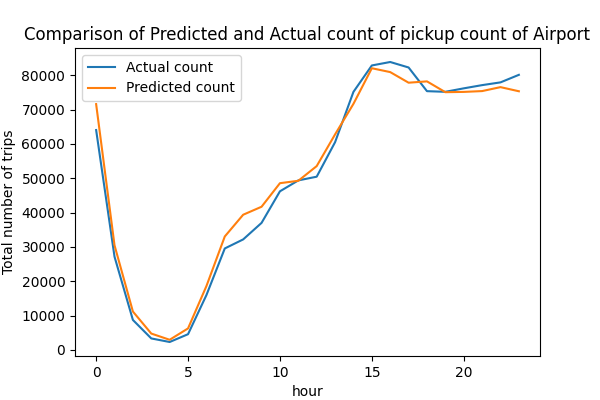
\includegraphics[width=\linewidth]{rfr_prediction_pickup_Airport.png}
     \caption{Comparison Actual vs Predicted count of Pickups in Airport}\label{Fig:rfr_pickup_airport}
   \end{minipage}\hfill
   \begin{minipage}{0.45\textwidth}
     \centering
     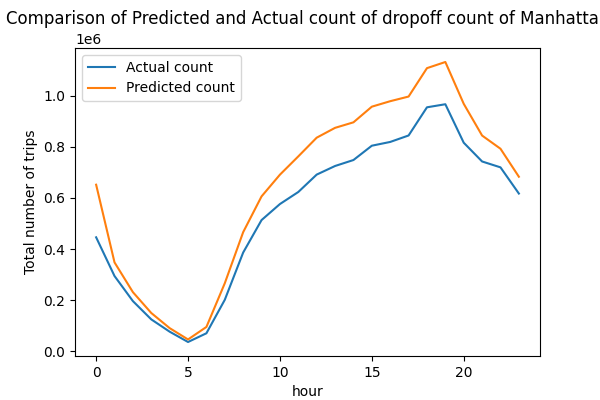
\includegraphics[width=\linewidth]{rfr_prediction_dropoff_Manhattan.png}
     \caption{Comparison of Actual vs Predicted count of Drop-offs in Manhattan}\label{Fig:rfr_dropoff_manhattan}
   \end{minipage}
\end{figure}

\section{Discussion}

\begin{table}[]
\centering
\begin{tabular}{|l|c|c|c|}
\hline
              & LR Pickup     & RFR Pickup      & \multicolumn{1}{l|}{RFR Drop-off} \\ \hline
Airport       & 730.12        & \textbf{345.53} & 69.75                             \\ \hline
Bronx         & \textbf{0.61} & 0.68            & 2.79                              \\ \hline
Brooklyn      & 3.38          & \textbf{3.22}   & 8.56                              \\ \hline
Manhattan     & 256.68        & \textbf{180.31} & 152.35                            \\ \hline
Staten Island & 0.08          & \textbf{0.05}   & 0.60                              \\ \hline
Queens        & 6.77          & \textbf{4.70}   & 6.82                              \\ \hline
\end{tabular}
\caption{Mean Squared Error for Linear Regression and Random Forest Regression}
\label{tab:mae_result}
\end{table}

According to Table \ref{tab:mae_result}, Random Forest Regressor has outperformed Linear Regression in almost every borough. The superior performance of the RFR model suggests that public transportation data has a more intricate impact on taxi demand than can be explained by a simple linear relationship. From Table \ref{tab:lr_result}, we can see that the R-squared values are very different for each borough. The airport region had the highest R-squared value of 0.927 while Staten Island had the lowest R-squared value of 0.244. Such a low R-squared value in Staten Island suggests that the variation in log(pickup count) was most likely due to factors not examined in this project. On the other hand, the total number of data points in Staten Island was very low compared to other boroughs. This could lead to Linear Regression not being able to capture the relationship due to insufficient data size. 

Figure \ref{Fig:rfr_pickup_airport} demonstrates that the RFR model was able to predict the pickup count of 2023 in the Airport region very accurately. On the other hand, the RFR model overestimated the drop-off count of 2023 in Manhattan. Although the model was able to capture the general pattern, it overestimated the trip count for other boroughs as well. This may be due to hidden factors that differentiate 2022 from 2023 data. From Table \ref{tab:mae_result}, we can see that RFR outperformed LR in almost every region. With very good MAE results, we can see that RFR was able to capture the complex relationship between public transport and taxi demand. In Queens, RFR was able to predict within 5 trips range. Considering the number of instances, this is a very good result. Similar to Linear Regression, each borough had different results. Lastly, RFR was able to predict drop-off counts with a mean absolute error of 70 in airport regions. Considering the good results, we conclude that there is a non-linear relationship between public transport and yellow taxi demands.

\section{Recommendations}

With a more accurate prediction of taxi demand, urban planners can make better-informed decisions regarding transportation infrastructure, traffic management, and allocation of resources. The insights gained from the RFR model can contribute to more efficient urban mobility strategies. Our low MAE model, relying solely on temporal features and public transport data, is able to predict future demands with high accuracy. For instance, Figure \ref{fig:lineplot_demand} demonstrated that taxi demand sees an increase on Wednesday and Thursday. Therefore, we recommend increasing public transport accessibility during that time in North Brooklyn. Figure \ref{fig:dropoff_choropleth} shows that North Brooklyn is a popular travel spot for taxi trips but Figure \ref{fig:public_transport} shows that the public transport is less accessible there compared to other areas. 

The accurate prediction of taxi demand can lead to improved commuter services by enabling taxi companies to optimize their fleet management and respond to fluctuations in demand effectively. This contributes to more convenient and reliable transportation options for the public. According to Figure \ref{fig:corr_matrix}, there exists a negative relationship between taxi service and public transport due to competition and transport availability. Therefore, we recommend taxi drivers and taxi companies start taking more trips around western Queens where public transport is less accessible than in Manhattan and Brooklyn. In addition, Figure \ref{fig:pickup_choropleth} shows that Queens is one of the popular pickup zones. 

\section{Conclusion}

This report has analysed the geospatial impact of public transport on yellow taxi demands using linear regression and ensemble methods as well as other analysis methods. According to the result, public transport data, combined with temporal data, can be used to predict yellow taxi demand with high performance.

The predictive power of these models not only provided accurate estimations of taxi demand but also highlighted the influence of public transportation services on commuting patterns. This study's findings can help public transport planners and taxi companies to better allocate their resources. 

Future research should consider importing socio-economic data, such as population and income level as well as additional data such as the number of tourist attraction spots. 

\clearpage

% BEGIN REFERENCES SECTION
\printbibliography

\end{document}